% Options for packages loaded elsewhere
\PassOptionsToPackage{unicode}{hyperref}
\PassOptionsToPackage{hyphens}{url}

  \PassOptionsToPackage{dvipsnames,svgnames,x11names}{xcolor}



%%%% Clase del documento y configuraciones generales de apariencia
\documentclass[
  %
  %
    a4paper,%
  %
  %
  %
    DIV=calc,%
  %
    abstract=true%
  ]{scrartcl}%

\usepackage{amsmath,amssymb}


\usepackage{iftex}

\ifPDFTeX                       % if pdflatex
  \usepackage[T1]{fontenc}
  \usepackage[utf8]{inputenc}
  \usepackage{textcomp}         % provide euro and other symbols
\else % if luatex or xetex
      \usepackage{unicode-math}   % this also loads fontspec
    \defaultfontfeatures{Scale=MatchLowercase}
  \defaultfontfeatures[\rmfamily]{Ligatures=TeX,Scale=1}
\fi

  
  \usepackage[]{Alegreya}

\ifPDFTeX\else    
  \usepackage{fontspec}
          
  
      \fi


\IfFileExists{upquote.sty}{\usepackage{upquote}}{}

\IfFileExists{microtype.sty}{
  \usepackage[]{microtype}
  \UseMicrotypeSet[protrusion]{basicmath} 
}{}

  \makeatletter
  \@ifundefined{KOMAClassName}{%    
    \IfFileExists{parskip.sty}{%
      \usepackage{parskip}
    }{
      \setlength{\parindent}{0pt}
      \setlength{\parskip}{6pt plus 2pt minus 1pt}}
  }{
    \KOMAoptions{parskip=half}}
  \makeatother


\usepackage{xcolor}





%%%% Configuración de tablas
  \usepackage{longtable,booktabs,array}
    \usepackage{calc} % for calculating minipage widths
  % Correct order of tables after \paragraph or \subparagraph
  \usepackage{etoolbox}
  \makeatletter
  \patchcmd\longtable{\par}{\if@noskipsec\mbox{}\fi\par}{}{}
  \makeatother
  % Allow footnotes in longtable head/foot
  \IfFileExists{footnotehyper.sty}{\usepackage{footnotehyper}}{\usepackage{footnote}}
  \makesavenoteenv{longtable}

%%%% Configuración de figuras
  \usepackage{graphicx}
  \makeatletter
  \def\maxwidth{\ifdim\Gin@nat@width>\linewidth\linewidth\else\Gin@nat@width\fi}
  \def\maxheight{\ifdim\Gin@nat@height>\textheight\textheight\else\Gin@nat@height\fi}
  \makeatother
  % Scale images if necessary, so that they will not overflow the page
  % margins by default, and it is still possible to overwrite the defaults
  % using explicit options in \includegraphics[width, height, ...]{}
  \setkeys{Gin}{width=\maxwidth,height=\maxheight,keepaspectratio}
  % Set default figure placement to htbp
  \makeatletter
  \def\fps@figure{htbp}
  \makeatother



\setlength{\emergencystretch}{3em} % prevent overfull lines
\providecommand{\tightlist}{%
  \setlength{\itemsep}{0pt}\setlength{\parskip}{0pt}}

  \setcounter{secnumdepth}{-\maxdimen} % remove section numbering




% Referencias con CSL

  \ifLuaTeX
    \usepackage[bidi=basic]{babel}
  \else
    \usepackage[bidi=default]{babel}
  \fi
      \babelprovide[main,import]{spanish}
      
      \babelprovide[import]{english}
      % get rid of language-specific shorthands (see #6817):
  \let\LanguageShortHands\languageshorthands
  \def\languageshorthands#1{}


% Customizaciones generales %%%%%%%%%%%%%%%%%%%%%

%%%% CARGA DE PAQUETES
\usepackage[export]{adjustbox}

% Cargar paquetes de íconos 
\usepackage{fontawesome5}
\usepackage{ccicons}

% Carga `setspace' para separación entre lineas (si no fue cargado)
\IfPackageLoadedTF{setspace}{}{\usepackage{setspace}}
% Carga `graphicx' si no fue cargado (dado que no se usa entorno pandoc para figures)
\IfPackageLoadedTF{graphicx}{}{\usepackage{graphicx}}
% Carga `etoolbox' 
\IfPackageLoadedTF{etoolbox}{}{\usepackage{etoolbox}}

% Carga de paquetes y configuraciones pedidas por el documento


%%%% COLORES CUSTOMIZADOS

\definecolor{verde_orcid}{RGB}{166,206,57}

%%%% CITAS LARGAS

% Definir estilo de citas largas (achica el tamaño)
\IfPackageLoadedTF{relsize}{}{\usepackage{relsize}}
\AtBeginEnvironment{quote}{\smaller}% Step font down one size relative to current font.

%%%% TABLAS Y FGURAS

% Agregado de \source y \notes para titulos secundarios de las tablas y figuras
\usepackage{caption}
\captionsetup{format=plain,labelsep=period,singlelinecheck=false,justification=centerlast,
              font={small,singlespacing,sf},labelfont={sc,bf},width=0.8\textwidth}
\newcommand{\source}[1]{\vspace{-9pt}\caption*{\footnotesize{\textit{Fuente:} {#1}}}}
\newcommand{\notes}[1]{\vspace{-9pt}\caption*{\footnotesize{\textit{Notas:} {#1}}}}



% Cambia denominación de "Cuadro" a "Tabla"
\renewcommand{\spanishtablename}{Tabla}

% Cambiar fuente y tamaño de letra para entorno de tablas (table)
\AtBeginEnvironment{tabular}{\sffamily\footnotesize}
\IfPackageLoadedTF{tabularray}{%
\AtBeginEnvironment{tblr}{\sffamily\footnotesize}}{}

%%%% ENCABEZADO DE PÁGINA
% Si utiliza clases de Koma-script debe utilizar el paquete 'scrlayer-scrpage'
% Si utiliza las clases estándar debe usar el paquete 'fancyhdr'
\usepackage[headsepline]{scrlayer-scrpage}
\usepackage[breakwords]{truncate}

\setkomafont{pagehead}{\normalfont\sffamily\small}

\ihead{\textit{\truncate{0.45\textwidth}{Documento de referencia para
\textasciitilde!gurí\_ (Gestor Unificado de formatos para Revistas de
Investigación)}}}
\ohead{\textbf{\textasciitilde!guri\_ \{An example journal\}}}

\setkomafont{pagefoot}{\normalfont\footnotesize}
\ifoot[\rule{0.4\textwidth}{0.5pt} \vskip 0.5em Publicación de \emph{guri}.
      ISSN-e: 0001-2000.\\
      Esta obra está bajo una licencia Creative Commons
Attribution-NonCommercial-ShareAlike 4.0 International
License (https://creativecommons.org/licenses/by-nc/4.0/).]{}
\cfoot[]{\pagemark}

% Definir primera página del artícul (si se utiliza paginación personalizada)

%%%% PÁGINA DE TÍTULO 
\setkomafont{titlehead}{\raggedright\sffamily\small}
\setkomafont{title}{\raggedright\sffamily}
\setkomafont{author}{\raggedright\sffamily\setlength{\tabcolsep}{0pt}}
\setkomafont{publishers}{\raggedright\sffamily\footnotesize}
\setkomafont{dedication}{\raggedright\sffamily\small}

\titlehead{%
  \textbf\textbf{PRESENTACIÓN DE LA
PROPUESTA}\hfill\textbf{\textasciitilde!guri\_ \{An example
journal\}}\\%
  \vspace{4pt}
  \hfill Vol. 10 Núm. 1 (2023)
  \\ \hfill DOI: \href{https://doi.org/10.1223/3344443.33221333}{10.1223/3344443.33221333}%
 }%

\title{Documento de referencia para \textasciitilde!gurí\_ (Gestor
Unificado de formatos para Revistas de Investigación)}

  \subtitle{\vspace{1em} \textit{Reference Document for
\textasciitilde!gurí\_ (Unified Format Manager for Research Journals)}}

\author{{\begin{tabular}[l]{@{}l@{}}%
  \large{Pablo {Serrati}}\textsuperscript{a;b} \href{https://orcid.org/0000-0001-5300-2243}{\textcolor{verde_orcid}{\faOrcid}}
\end{tabular}}%
}
    
\date{}

\publishers{
  \vspace{1em}
  \textsuperscript{a} Consejo Nacional de Investigaciones Científicas y
Técnicas (CONICET), Argentina.\\\textsuperscript{b} Universidad de
Buenos Aires, Facultad de Ciencias Sociales, Instituto de
Investigaciones Gino Germani, Argentina.
  \\ \vspace{1em} \textit{Recibido:} 2 de Mayo de 2023; \textit{Aceptado:} 10 de Enero de 2024.\\%
}




%%% Credit, Ack and app Enviroment

\newenvironment{Credit}[1][Declaración de contribuciones de autoría (CRediT)]
    {\subsection*{#1}
    \sffamily\small}

\newenvironment{Ack}{\begin{Credit}[Agradecimiento]}{\end{Credit}}%

\newenvironment{app}{\newpage}{}
\ifLuaTeX
  \usepackage{selnolig}  % disable illegal ligatures
\fi






\usepackage{bookmark}

\IfFileExists{xurl.sty}{\usepackage{xurl}}{} % add URL line breaks if available
\urlstyle{same}



\hypersetup{
      pdftitle={Documento de referencia para \textasciitilde!gurí\_ (Gestor Unificado de formatos para Revistas de Investigación)},
        pdfauthor={Pablo Serrati},
    pdfsubject={\textasciitilde!guri\_ \{An example
journal\} - Volume: 10  - Issue: 1  (2023) a201 doi: 10.1223/3344443.33221333},
      pdflang={es-ES},
        pdfkeywords={guri, modelo de plantilla, ejemplo},
    pdfinfo={
          DOI={10.1223/3344443.33221333},
              abstract={Este documento describe de modo resumido las
características principales de \textasciitilde!gurí. A su vez
ejemplifica con la plantilla modelo de Word el modo en que deben
definirse los diferentes bloques dentro del texto.},
        journal=\textasciitilde!guri\_ \{An example journal\}
      },
  % Define color de links
      colorlinks=true,
    linkcolor={CadetBlue},
    filecolor={CadetBlue},
    citecolor={CadetBlue},
    urlcolor={CadetBlue},
  pdfcreator={LaTeX via pandoc \& \textasciitilde!guri\_}}

%%%% Inicio de documento

\begin{document}
  
  
  \maketitle

  
    
    
    \begin{abstract}

      \noindent{Este documento describe de modo resumido las
características principales de \textasciitilde!gurí. A su vez
ejemplifica con la plantilla modelo de Word el modo en que deben
definirse los diferentes bloques dentro del texto.}

      \nopagebreak

      \noindent\sffamily\textit{Palabras claves: guri; modelo de
plantilla; ejemplo}.%

    \end{abstract}
    
        \begin{otherlanguage}{english}

      \begin{abstract}      
 
        \noindent{This document summarises the main features of
\textasciitilde!gurí. It also uses the Word template to illustrate how
the different blocks within the text should be defined.}

        \nopagebreak

        \noindent\sffamily\textit{Keywords: guri; template; example}.%

      \end{abstract}
    \end{otherlanguage}
      

    
    
      
  
  
  \section{Descripción general de la propuesta (Heading
  1)}\label{descripciuxf3n-general-de-la-propuesta-heading-1}

  La herramienta \textasciitilde!gurí\_ es un flujo de trabajo y un
  conjunto de herramientas que facilitan una automatización del proceso
  de generación de documentos finales para revistas científicas a partir
  de documentos obtenidos en la etapa de `corrección de pruebas'. La
  herramienta se basa en el uso de Pandoc como herramienta de conversión
  entre formatos, a la cual se incorpora un conjunto de filtros Lua y
  plantillas personalizadas, así como un flujo de trabajo, lo cual
  permite en su conjunto la creación de los documentos finales.

  \begin{figure}
  \centering
  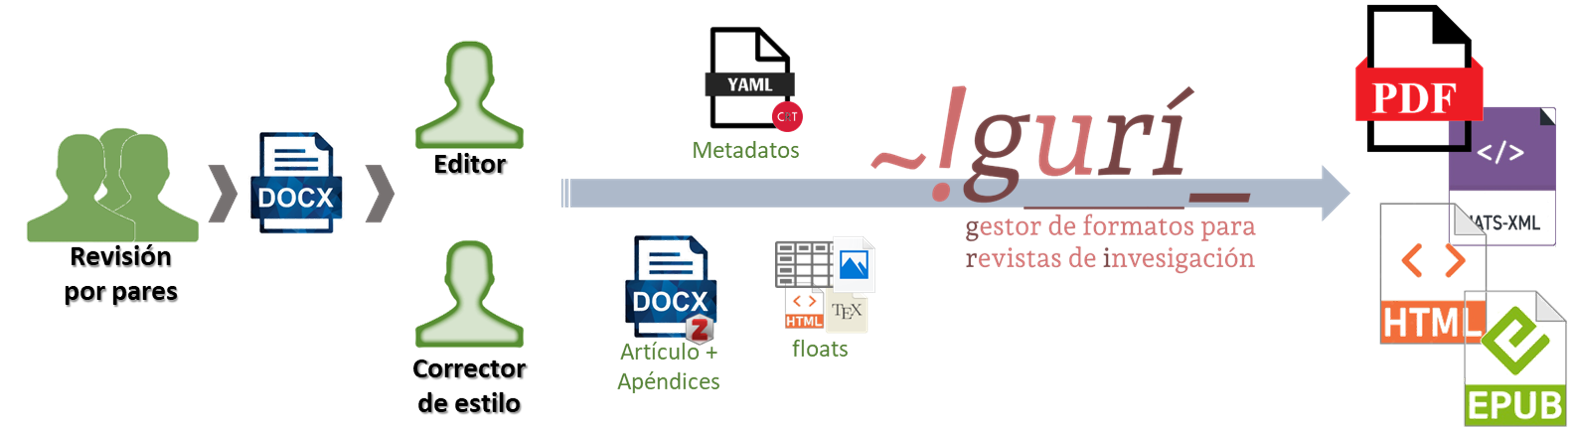
\includegraphics[width=0.9\textwidth]{./float/FIG_01}
  \caption{Esquema general de gurí}
  \source{Elaboración propia (ver https://github.com/estedeahora/guri)}
  \label{FIG_01}
  \end{figure}

  En términos resumidos, la propuesta propone esquematizar y separar los
  principales elementos que componen un artículo científico. En
  particular, la propuesta considera el hecho de que muchas revistas
  utilizan como base de sus flujos de trabajos documentos docx.

  \section{Descripción de las dependencias de software (Heading
  1)}\label{descripciuxf3n-de-las-dependencias-de-software-heading-1}

  Esta herramienta se basa en el uso de
  \href{https://pandoc.org/}{Pandoc} (versión 3.1.10 o superior) como
  herramienta de conversión entre formatos. Si no tiene instalado este
  software deberá hacerlo directamente de la página oficial.

  También es necesario instalar alguna versión de
  \href{https://cran.r-project.org/}{R} (recomendable versión 4.3 o
  superior), que es el encargado de coordinar el proceso de
  conversiones. También es necesario tener instalada alguna distribución
  de LaTeX. A las personas con poca experiencia en el uso de LaTeX,
  recomendamos utilizar la distribución
  \href{https://yihui.org/tinytex/}{tinitex}, por su integración con R y
  la facilidad para manejar las dependencia de paquetes. De hecho, esta
  versión se utiliza de forma predeterminada para la generación de
  archivos PDF.

  \section{Ejemplo de marcado y uso de estilos (Heading
  1)}\label{ejemplo-de-marcado-y-uso-de-estilos-heading-1}

  \subsection{Descripción de la lógica de marcado (Heading
  2)}\label{descripciuxf3n-de-la-luxf3gica-de-marcado-heading-2}

  Una vez que haya hecho las configuraciones generales de su revista,
  deberá dar formato a cada uno de los artículos. Para ello debe
  utilizar una plantilla de docx (similar a la que se usa en este
  ejemplo). Para esta tarea debe utilizar los ``Estilos'' de párrafo y
  de ``caracter'' que están predefinidos en la plantilla (dentro de
  \emph{Microsoft Word} se encuentran la lista de estilos en la pestaña
  ``Inicio'' -\textgreater{} ``Estilos''). Es importante remarcar que no
  se trata de formatear el texto de manera similar a estos estilos, sino
  de usar los estilos predefinidos. Si usted genera estilos
  personalizados estos no serán tenidos en cuenta (o se usarán de formas
  impredecibles).

  En los apartados siguiente se ejemplifican los estilos que soporta
  \textasciitilde!gurí\_.

  \subsection{Ejemplificación de los principales bloques (Heading
  2)}\label{ejemplificaciuxf3n-de-los-principales-bloques-heading-2}

  Este es un párrafo de estilo normal del cuerpo. Para ellos se debe
  utilizar ``Body Text'' o ``Texto independiente'' (según su
  configuración regional). Dentro de este párrafo pueden existir
  diferentes tipos de ``estilos de carácter'', como \emph{cursiva} o
  \textbf{negritas} (aunque esta última no es recomendable por una
  cuestión estética). También puede incluir tipografías monoespaciadas
  (por ejemplo, para código informático) utilizando el estilo de
  caracter
  \texttt{Verbatim\textasciigrave{}\textasciigrave{}\ \textasciigrave{}\textasciigrave{}Char\textasciigrave{}\textasciigrave{}\ o\ \textasciigrave{}\textasciigrave{}Source\textasciigrave{}\textasciigrave{}\ \textasciigrave{}\textasciigrave{}code}
  (dependiendo de su configuración de idioma).

  A su vez, puede usar \href{http://example.com}{Hipervínculos o
  hyperlink}, estilos que se formatearan automáticamente si establece
  una referencia al texto. De igual manera las notas al pie o
  ``Footnote'' se formatearán de forma automática si usted genera una
  nota con \emph{Microsoft Word}.\footnote{Footnote Text. No es
    necesario utilice un estilo específico para las notas al pie, sino
    que podrá usar estilo ``Texto independiente''.}

  También puede utilizar: listas (numeradas y no numeradas), bloques de
  citas, ecuaciones y definiciones y bloques de código. Para hacer una
  ejemplificación del uso de los diferentes niveles de título, vamos a
  abordar cada aspecto en un título propio.

  \subsubsection{Listas (Heading 3)}\label{listas-heading-3}

  Puede incluir listas numeradas (y listas anidadas) mediante el uso de
  las funciones de \emph{Microsoft Word}:

  \begin{enumerate}
  \def\labelenumi{\arabic{enumi}.}
  \item
    Elemento 1

    \begin{enumerate}
    \def\labelenumii{\alph{enumii}.}
    \item
      Esto es un aspecto del elemento 1

      \begin{enumerate}
      \def\labelenumiii{\roman{enumiii}.}
      \tightlist
      \item
        Esto es una lista profundamente anidada (no recomendable)
      \end{enumerate}
    \item
      Esto es un segundo aspecto del elemento 1
    \end{enumerate}
  \item
    Elemento 2
  \end{enumerate}

  También puede incluir listas sin numerar de la siguiente manera:

  \begin{itemize}
  \item
    Esto es una lisa de elementos sin numerar.

    \begin{itemize}
    \item
      Acá la lista está anidada
    \item
      Con dos elementos\\
      Si desea agregar más de un párrafo dentro de un bullet use el
      salto de párrafo ``blando'' (shift + enter)
    \end{itemize}
  \item
    Esto es el segundo elemento.
  \end{itemize}

  Este es un fragmento de texto normal generado para mostrar cómo se
  intercalan párrafos de diferente tipo (por lo tanto, utiliza como
  estilo ``Texto independiente'' o ``Body Text''). El resto del párrafo
  es sólo texto aleatorio: Lorem ipsum dolor sit amet, consectetur
  adipiscing elit. Aliquam posuere dolor elementum leo feugiat
  pellentesque vitae porttitor diam. Ut tempus magna et velit suscipit
  finibus quis quis lacus. Duis euismod velit nec augue porttitor
  dictum. Vivamus efficitur, lorem eu varius tempus, tortor augue
  accumsan risus, in lacinia diam leo vel massa. Vivamus tempus sapien
  ut ante imperdiet ullamcorper.

  \subsubsection{Bloques de texto o cita larga (Heading
  3)}\label{bloques-de-texto-o-cita-larga-heading-3}

  Es posible utilizar el estilo ``Block text'' o ``Texto de bloque''
  para identificar un bloque de cita larga como el siguiente:

  \begin{quote}
  Esto es una cita larga (o ``Block Text''). Habitualmente puede ser una
  cita de más de 40 palabras de un texto o bien una entrevista. Si usted
  posee un bloque con varios párrafos, puede mantenerlos ``unidos''
  utilizando ``saltos de línea blandos'' (en \emph{Microsoft Word} esto
  se consigue con shift + enter).\\
  Esto es un ejemplo de salgo de línea blando.

  Por otra parte, si se trata de diferentes bloques (por ejemplo:
  diferentes entrevistados), debe colocar un salto de párrafo ``duro''
  (enter). De esta manera, cada bloque será separado por un espacio
  mayor.
  \end{quote}

  Algo de texto aleatorio para separar: Phasellus vulputate aliquet
  scelerisque. Nullam vel tellus eget nisi dapibus auctor. Vivamus et
  dolor ac quam vestibulum iaculis. Curabitur varius elit in
  pellentesque fermentum. Cras pharetra mi id nibh laoreet vulputate.
  Integer tristique facilisis sapien ac ornare. Integer pretium ac eros
  et sollicitudin.

  \subsubsection{Ecuaciones, fórmulas y definiciones (Heading
  3)}\label{ecuaciones-fuxf3rmulas-y-definiciones-heading-3}

  Para incluir una fórmula matemática dentro del texto puede hacerlo
  mediante el uso del editor de fórmulas de \emph{Microsoft Word}. Estas
  pueden estar incluidas dentro del cuerpo del texto con el formato
  normal \(y = a + bx + cx^{2}\) o bien en párrafo aparte:

  \[y = a + bx + cx^{2}\]

  En algunos casos en los que tenga ``definiciones'' en párrafo aparte
  (al estilo matemático) puede utilizar los estilos ``Definition Term''
  (para el nombre de lo que va a definir) y ``Definition'' (para la
  definición en sí). Esto sería un ejemplo:

  \begin{description}
  \item[Término a definir]
  Esta es la definición del término anterior. La misma explica qué
  quiere decir lo que definió anteriormente
  \end{description}

  Más texto aleatorio: Curabitur nec odio vitae neque viverra ornare non
  posuere elit. Quisque placerat imperdiet velit, vel consequat nisl
  vestibulum ac. Fusce vitae velit et velit vestibulum volutpat eu nec
  eros.

  \subsubsection{Bloques de código (Heading
  3)}\label{bloques-de-cuxf3digo-heading-3}

  A su vez, puede generar un bloque de código utilizando un párrafo sólo
  con ``Surce code'' como se hace a continuación:

\begin{verbatim}
for i in Source_code
  print (i)
  print(“hola mundo”)
end
\end{verbatim}

  Algo de texto aleatorio: Lacinia quis vel eros donec ac odio tempor.
  Eu turpis egestas pretium aenean pharetra magna ac. Nec nam aliquam
  sem et. Eu sem integer vitae justo. A pellentesque sit amet porttitor
  eget dolor. Tortor vitae purus faucibus ornare suspendisse sed nisi
  lacus sed. Vitae tempus quam pellentesque nec nam aliquam sem. Leo vel
  fringilla est ullamcorper eget.

  \subsection{Marcador de elementos flotantes (Heading
  2)}\label{marcador-de-elementos-flotantes-heading-2}

  Un aspecto particular de la propuesta es que los elementos flotantes
  (tablas o figuras) deben ser identificados con marcadores especiales.
  Para marcar elementos los flotantes debe utilizar el siguiente
  marcador:

  \begin{figure}
  \centering
  
\includegraphics[width=0.9\textwidth]{./float/FIG_02}
  \caption{Ejemplo de figura (logo gurí)}
  \source{Elaboración propia (ver https://github.com/estedeahora/guri)}
  \label{FIG_02}
  \end{figure}

  No es necesario que utilice el resaltado, aunque esto puede ayudarle
  para la edición de documentos. Tenga en cuenta que este marcador
  utiliza saltos de línea débiles (ctr + enter) entre sus diferentes
  líneas. Técnicamente es posible todo en una línea, separando los
  elementos del mismo por un espacio, pero es más difícil de leer. Por
  otra parte, tenga en cuenta que entre el símbolo igual (``='') y el
  contenido del elemento no debe haber ningún espacio (o se producirá un
  error en el documento final). Si desea hacer referencia a un elemento
  flotante, puede hacerlo utilizando como marcador el siguiente marcador
  \hyperref[FIG_02]{Figura 2} (nuevamente el resaltado es sólo para
  simplificar su ubicación durante la tarea y no será visible en la
  versión final). Tenga en cuenta que esta marca insertará la palabra
  ``Figura'' / ``Tabla'' y el número de la misma, con un hipervínculo a
  la misma.

  Recuerde que cada una de estas figuras o tablas deben estar en una
  carpeta con el nombre ``float'' (dentro de la carpeta del artículo) y
  deben tener el mismo nombre que indica en el bloque de marcación (en
  el campo ``include''). Este nombre no deberá incluir la extensión de
  formato del archivo (png, jpg, etc.). Por su parte, si el elemento
  flotante es una tabla, deberá proveer las mismas en formato tex (para
  la salida en pdf) y html (usada en la salida xml-jats y html).

  \subsection{El uso de la herramienta de ``control de cambios''
  (Heading
  2)}\label{el-uso-de-la-herramienta-de-control-de-cambios-heading-2}

  Usted puede introducir cambios con la herramienta ``control de
  cambios'' de \emph{Microsoft Word}, de manera que el documento final
  será

  \section{Comentarios finales}\label{comentarios-finales}

  Tenga en cuenta que este documento no es un manual, sino sólo un
  ejemplo de cómo puede realizarse la preparación de documentos finales
  en \emph{Microsoft Word}. Para una explicación de la instalación,
  configuración global de su revista y del proceso de preparación de
  documentos debe leer los documentos disponibles en el repositorio:
  \url{https://github.com/estedeahora/guri/tree/main/manual}

  Recuerde que este software es distribuido bajo una
  licencia~\href{http://creativecommons.org/licenses/by-nc-sa/4.0/}{Creative
  Commons Attribution-NonCommercial-ShareAlike 4.0 International
  License}. El software no ofrece garantía de ningún tipo. Se solicita
  que si su revista utiliza esta herramienta como parte de su proceso
  editorial agregue el siguiente texto dentro de su página web
  (habitualmente dentro de la sección de `política editorial') en los
  diferentes idiomas que utilice en la revista:

  \begin{quote}
  \emph{Español:}\\
  Los documentos finales de esta revista fueron generados
  utilizando~\href{https://github.com/estedeahora/guri}{\textasciitilde!guri\_}.

  \emph{English:}\\
  The final documents of this journal were generated
  using~\href{https://github.com/estedeahora/guri}{\textasciitilde!guri\_}.

  \emph{Português:}\\
  Os documentos finais desta revista foram gerados
  usando~\href{https://github.com/estedeahora/guri}{\textasciitilde!guri\_}.
  \end{quote}

  \begin{Credit}

  \phantomsection\label{Credit}
  \textbf{Serrati:} Conceptualización (Conceptualization); Curación de
  datos (Data curation); Análisis formal (Formal Analysis); Adquisición
  de Financiamiento (Funding acquisition); Investigación
  (Investigation); Metodología (Methodology); Administración de proyecto
  (Project administration); Recursos (Resources); Software (Software);
  Supervisión (Supervision); Validación (Validation); Visualización
  (Visualization); Redacción - preparación del borrador original
  (Writing -- original draft); Redacción - revisión y edición (Writing
  -- review \& editing).

  \end{Credit}

    
  %%%% Referencias bibliográficas
  
  
    
\end{document}
